\documentclass[12pt]{article}
\usepackage{amsmath}
\usepackage{amssymb}
\usepackage[letterpaper,top=0.75in,bottom=0.75in,left=0.75in,right=0.75in,centering]{geometry}
%\usepackage{fancyhdr}
\usepackage{enumerate}
%\usepackage{lastpage}
\usepackage{multicol}
\usepackage{graphicx}
\usepackage{vwcol}

\reversemarginpar

%\pagestyle{fancy}
%\cfoot{}
%\lhead{Math 1560}\chead{Test \# 1}\rhead{May 18th, 2017}
%\rfoot{Total: 10 points}
%\chead{{\bf Name:}}
\newcommand{\points}[1]{\marginpar{\hspace{24pt}[#1]}}
\newcommand{\skipline}{\vspace{12pt}}
%\renewcommand{\headrulewidth}{0in}
\headheight 30pt

\newcommand{\di}{\displaystyle}
\newcommand{\abs}[1]{\lvert #1\rvert}
\newcommand{\len}[1]{\lVert #1\rVert}
\renewcommand{\i}{\mathbf{i}}
\renewcommand{\j}{\mathbf{j}}
\renewcommand{\k}{\mathbf{k}}
\newcommand{\R}{\mathbb{R}}
\newcommand{\aaa}{\mathbf{a}}
\newcommand{\bbb}{\mathbf{b}}
\newcommand{\ccc}{\mathbf{c}}
\newcommand{\dotp}{\boldsymbol{\cdot}}
\newcommand{\bbm}{\begin{bmatrix}}
\newcommand{\ebm}{\end{bmatrix}}                   
                  
\begin{document}


\author{Instructor: Sean Fitzpatrick}
\thispagestyle{empty}
\vglue1cm
\begin{center}
{\bf MATH 1560 - Tutorial \#9 Solutions}\
\end{center}

Additional Practice:
\begin{enumerate}
\item Compute the derivative:
\begin{enumerate}
\item $\di\frac{d}{dx}(e^x\cos(x)) = e^x(\cos(x)-\sin(x))$ (product rule)
\item $\di \frac{d}{dx}\sec(x) = \sec(x)\tan(x)$
\item $\di\frac{d}{dx}(1+x^2)^{12} = 24x(1+x^2)^{11}$ (chain rule)
\item $\di\frac{d}{dx}\frac{e^x}{x} = \frac{e^x(x-1)}{x^2}$ (quotient rule)
\item $\di\frac{d}{dx}\ln(\sin(x)) = \frac{\cos(x)}{\sin(x)}=\cot(x)$ (chain rule)
\item $\di\frac{d}{dx}2\sin^4(x)=8\sin^3(x)\cos(x)$ (chain rule)
\end{enumerate}

\item Evaluate the immediate integral:

\begin{enumerate}
\item $\di \int(3x^2+1+\frac1x+\frac{1}{x^2})\,dx = x^3+x+\ln\abs{x}-\frac1x +C$
\item $\di \int x(x^2+5)^4\,dx = \frac{1}{10}(x^2+5)^5+C$
\end{enumerate}

\item Given $y(x)=\pi x(50-x)$, solve $y'(x)=0$.

$y(x) = (50 x- x^2)$, so  $y'(x) = \pi(50-2x)=2\pi(25-x)$, and $y'(x)=0$ for $x=25$.

\item Given $D(x) = \sqrt{5x^2+20x+25}$, solve $D'(x)=0$

Since $\di D'(x) =\frac{10x+20}{2\sqrt{5x^2+20x+25}}=\frac{5(x+2)}{\sqrt{5x^2+20x+25}}$, we get $D'(x)=0$ when $x=-2$.
\end{enumerate}




\newpage
%\thispagestyle{empty}



  \begin{enumerate}
    \item Compute the derivative:
  
    \begin{enumerate}
    \item $\di\frac{d}{dx}\sin(1/x) = -\frac{1}{x^2}\cos(1/x)$ (chain rule)
    
 
    
    \item $\di\frac{d}{dx}\ln(A+Bx^4) = \frac{4Bx^3}{A+Bx^4}$ (chain rule) 
    
    
    \item $\di\frac{d}{dx}\sqrt{1+x^4} = \frac{2x^3}{\sqrt{1+x^4}}$ (chain rule)
    
    \item $\di\frac{d}{dx}\ln[f(x)g(x)] = \frac{d}{dx}(\ln(f(x))+\ln(g(x))=\frac{f'(x)}{f(x)}+\frac{g'(x)}{g(x)}$ (chain rule)
    
   
    \end{enumerate} 
    \item Evaluate the integral:
    \begin{enumerate}
    \item $\di\int 10\cos(x)\sin^4(x)\,dx = 2\sin^5(x)+C$
    
    
    \item $\di\int 6x\sqrt{x^2+7}\,dx = 2(x^2+7)^{3/2}+C$
    
    
    \item $\di\int\frac{2x+\cos(x)}{x^2+\sin(x)}\,dx = \ln\abs{x^2+\sin(x)}+C$
    
    
    \item $\di\int\frac{dx}{x\ln^3\abs{x}}= -\frac{1}{2\ln^2\abs{x}}+C$
    \end{enumerate}
    
    
    \item Given $V(r)=\pi H\left((r^2-\frac{r^3}{R}\right)$, with $H$ and $R$ constants, solve $V'(r)=0$.

   Since $V'(r) = \pi H\left(2r-\dfrac{3r^2}{R}\right) = \dfrac{\pi H}{R} r(2R-3r)$, we have $V'(r)=0$ for $r=0$ or $R=\dfrac{2R}{3}$.
   
   
   \item Given $y(x)=e^{-x^2}$, solve $y''(x)=0$.
   
   We have $y'(x) = -2xe^{-x^2}$, so 
   \[
   y''(x) = -2e^{-x^2}+4x^2e^{-x^2}=2e^{-x^2}(2x^2-1)=2e^{-x^2}(\sqrt{2}x-1)(\sqrt{2}x+1),
   \]
   so $y''(x)=0$ for $x = \pm\dfrac{1}{\sqrt{2}}$.
   
   \item Find the minimum possible cost for a square based, 12 litre box, with lid, if the base material costs \$0.20 per square centimetre, and the sides and lid cost \$0.10 per square centimetre. (Recall that 1 litre = 1000 cubic centimetres.)

  \begin{multicols}{2}
  \begin{center}
  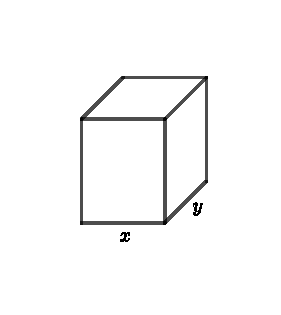
\includegraphics[width=0.3\textwidth]{Tut9-5sol}
  \end{center}
  
\columnbreak  
  
  Let $x$ be the length of one side of the base, and $y$ the height, as shown. Then the volume of the box is $V=x^2y=12000$. The cost of the base is given by $0.2x^2$, the lid costs $0.1x^2$, and the four sides cost $4(0.1)xy=0.4xy$, giving a total cost of $C=0.3x^2+0.4xy$.
 \end{multicols}
  Using the volume constraint to write $y=12000/x^2$, we get
  \begin{align*}
  C(x) &= 0.3x^2+\frac{0.4x(12000)}{x^2} = 0.3x^2+\frac{4800}{x}\\
  C'(x) & = 0.6x-\frac{4800}{x^2} = \frac{0.6x^3-4800}{x^2} = \frac{0.6(x^3-8000)}{x^2},
  \end{align*}
  so $C'(x) = 0$ when $x^3=8000$, or $x=20$. We can see that $C'(x)<0$ for $x<20$ and $C'(x)>0$ for $x>20$ so this is a local minimum. (And the global minimum: it's the only critical point, and $C(x)$ becomes very large if $x$ is either very small or very large.)
  
  When $x=20$, we find that $y=30$, and the total cost is
  \[
  C(20) = (\$ 0.3)(20)^2+\frac{\$ 4800}{20} = \$ 3.60.
  \]
  
  
  \item Find the maximum possible volume of a circular cylinder that can be put inside a sphere of radius $R$.
  
  Recall that the volume of a cylinder of radius $R$ and height $H$ is $\pi R^2H$.
  
  \medskip
  
  \begin{multicols}{2}
  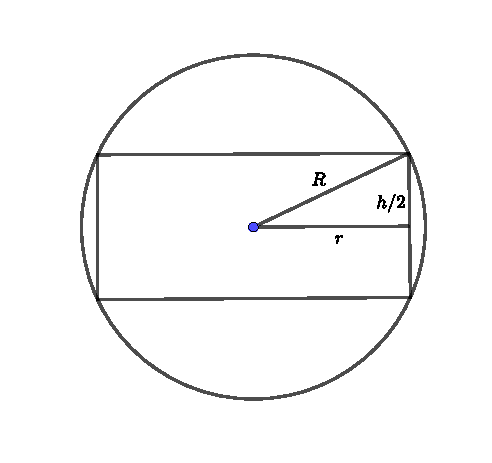
\includegraphics[width=\columnwidth]{Tut9-6sol}
 
  \columnbreak
  
  The diagram to the left shows a cross-section of the situation: a cylinder of height $h$ and radius $r$ sits inside a sphere of radius $R$. The cylinder must be centred with respect to the sphere, or we could shift it over, and increase its size.
  
  We can see that the values $r$ and $h$ must satisfy $r^2+(h/2)^2=R^2$.
   \end{multicols}
   Now, the volume of the cylinder is given by $V=\pi r^2h$, and since $r^2 = R^2-\dfrac{h^2}{4}$, we get
   \begin{align*}
   V(h) & = \pi\left(R^2 h-\frac{h^3}{4}\right)\\
   V'(h) & = \pi \left(R^2-\frac34 h^2\right) = \pi \left(R-\frac{\sqrt{3}}{2}h\right)\left(R+\frac{\sqrt{3}}{2}h\right),
   \end{align*}
   so $V'(h)=0$ when $h = \pm \dfrac{2R}{\sqrt{3}}$. The negative root is rejected since we must have $h>0$, and we can also check that this is the critical number which gives the desired maximum. The maximum volume is therefore
   \[
   V(2R/\sqrt{3}) = \frac{4\pi R^3}{3\sqrt{3}}.
   \]
    \end{enumerate}
\end{document}